\documentclass{article}
\usepackage{tikz}
\usetikzlibrary{quotes}
\tikzset{
    seagull/.pic={
    % Code for a "seagull". Do you see it?...
    \draw (-3mm,0) to [bend left] (0,0) to [bend left] (3mm,0);
    }
}
\tikzset{
    seagull2/.pic={
    % Code for a "seagull". Do you see it?...
    \coordinate (-left wing) at (-3mm,0);
    \coordinate (-head) at (0,0);
    \coordinate (-right wing) at (3mm,0);
    \draw (-left wing) to [bend left] (0,0) (-head) to [bend left] (-right wing);
    }
}
\tikzset{
    my pic/.pic = {
        \path [pic actions] (0,0) circle[radius=3mm];
        \draw (-3mm,-3mm) rectangle (3mm,3mm);
    }
}
\begin{document}
\tikz \fill [fill=blue!20]
(1,1)
-- (2,2) pic {seagull}
-- (3,2) pic {seagull}
-- (3,1) pic [rotate=30] {seagull}
-- (2,1) pic [red] {seagull};

\tikz {
\path (0,0) pic [pic type = seagull]
(1,0) pic {seagull};
}

\tikz [scale=2] {
\pic at (0,0) {seagull};
\pic at (1,0) [transform shape] {seagull};
}

\tikz [rotate=30] {
\pic at (0,0) {seagull};
\pic at (1,0) [rotate=90] {seagull};
}

% \tikz \draw (0,0) to [bend left]
% pic [near start] {seagull}
% pic {seagull}
% pic [sloped, near end] {seagull} (4,0)

% \tikz \pic [pics/code={\draw (-3mm,0) to[bend left] (0,0)
% to[bend left] (3mm,0);}]
% {}; % no pic type specified

\tikz \draw (0,0) .. controls(1,0) and (2,1) .. (3,1)
foreach \t in {0, 0.1, ..., 1} {
pic [pos=\t] {code={\draw circle [radius=2pt];}}
};

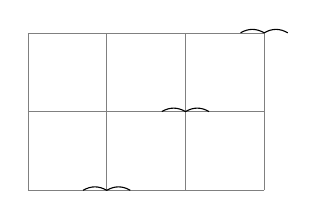
\begin{tikzpicture}
\draw [help lines] (0,0) grid (3,2);
\pic at (1,0) {seagull};
\path (2,1) pic {seagull};
\pic [at={(3,2)}] {seagull};
\end{tikzpicture}

\tikz \pic {my pic}; \space
\tikz \pic [red] {my pic}; \space
\tikz \pic [draw] {my pic}; \space
\tikz \pic [draw=red] {my pic}; \space
\tikz \pic [draw, shading=ball] {my pic}; \space
\tikz \pic [fill=red!50] {my pic};

\tikz \fill [fill=blue!20]
(1,1)
-- (2,2) pic [behind path] {seagull}
-- (3,2) pic {seagull}
-- (3,1) pic [rotate=30] {seagull}
-- (2,1) pic [red, behind path] {seagull};

\tikz \pic foreach \x in {1,2,3} at (\x,0) {seagull};

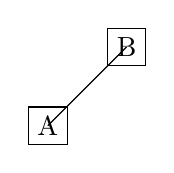
\begin{tikzpicture}[every node/.style={draw}]
\draw (0,0) node {A} -- (1,1) node {B};
\end{tikzpicture}

\tikz {
\pic (Emma) {seagull2};
\pic (Alexandra) at (0,1) {seagull2};
\draw (Emma-left wing) -- (Alexandra-right wing);
}

\tikzset{
pics/my circle/.style = {
background code = { \fill circle [radius=#1]; }
}
}
\tikz [fill=blue!30]
\draw (0,0) pic {my circle=2mm} -- (1,1) pic {my circle=5mm};
\end{document}